\begin{frame}{Background: Merger}
    \begin{itemize}
        \item Two governing bodies of Tokyo merged into a single body (Tokyo-To) in 1943.

        Tokyo-Fu: Central areas of Tokyo. Governor assigned from Federal government.
        
        Tokyo-Shi: Adjacency of Tokyo-Fu. Governor appointed from the municipal council.

        \

        \item Federal government ordered the merger to increase control over human/capital resources in Tokyo to support the war.
        
        \

        \item Managers in Tokyo-Shi were replaced by managers or high-ranked employees from the Tokyo-Fu.

    \end{itemize}
\end{frame}

\begin{frame}{Map}
    \begin{figure}
        \centering
        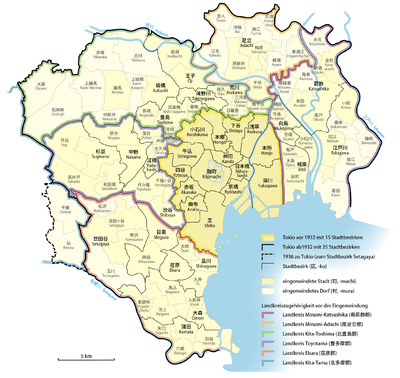
\includegraphics[height = 0.8\textheight]{Background/Map.png}
        \caption{Central Darker Yellow area is Tokyo-Fu, Surrounding light yellow area is Tokyo-Shi}
        \label{fig:enter-label}
    \end{figure}
\end{frame}

\begin{frame}{Background: Merger}
    \begin{itemize}
        \item The merger resulted in a mass layoff of employee in both organizations.

        \begin{enumerate}
            \item In average, 80\% of workers in a office in Tokyo-Fu were laid off.
            \item In average, 70\% of workers in a office in Tokyo-Shi were laid off.
        \end{enumerate}

        \

        \item In previously Tokyo-Shi offices, the number of incoming employees from Tokyo-Fu dictated the number of position to fill.

        Positions were filled by new hires and previous Tokyo-Fu employees.

        \

        \item TokyoTo retained experienced workers from TokyoShi to ease frictions in operations.
    \end{itemize}
\end{frame}

\begin{frame}{Retention for Tokyo-Shi}
    \begin{figure}
        \centering
        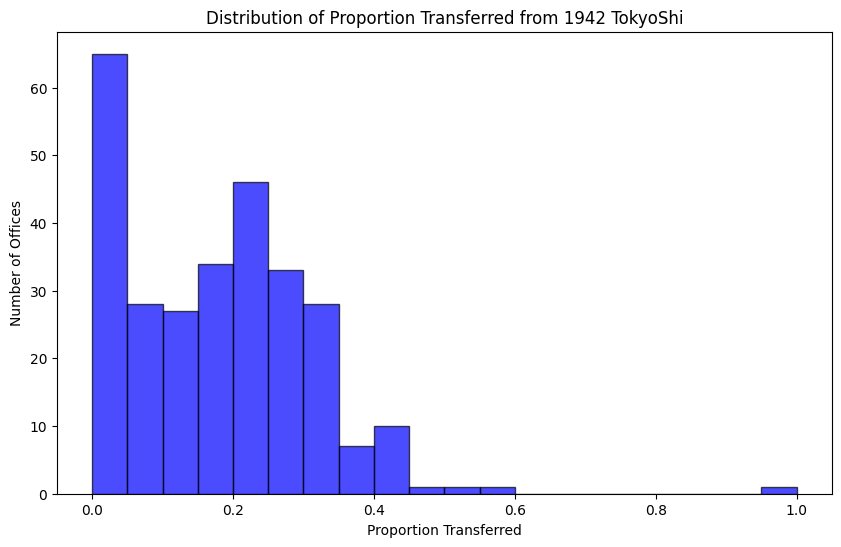
\includegraphics[width = \textwidth]{Background/TokyoShiTransfer.png}
        \label{fig:enter-label}
    \end{figure}
\end{frame}

\begin{frame}{Retention for Tokyo-Shi}
    \begin{figure}
        \centering
        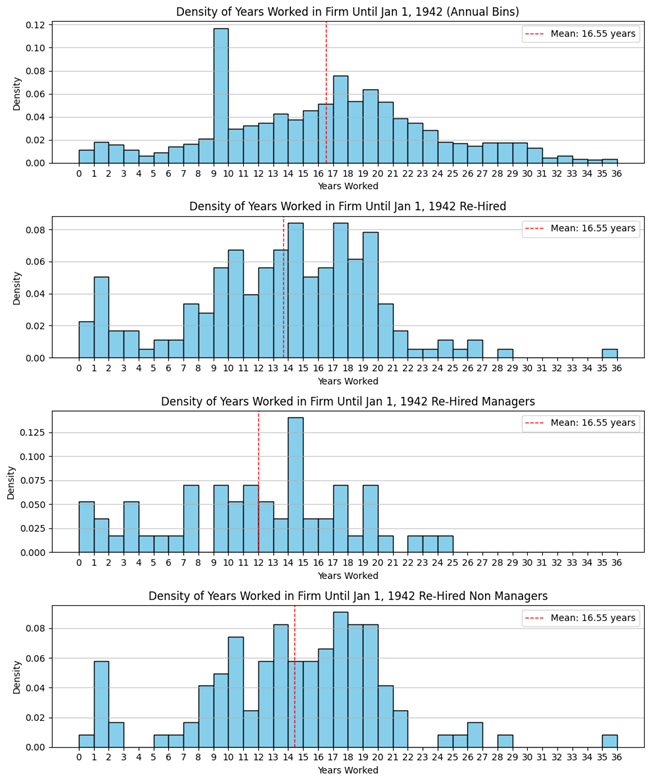
\includegraphics[height = 0.9\textheight]{Background/RehiringTokyoShi.png}
        \label{fig:enter-label}
    \end{figure}
\end{frame}


\begin{frame}{Retention for Tokyo-Fu}
    \begin{figure}
        \centering
        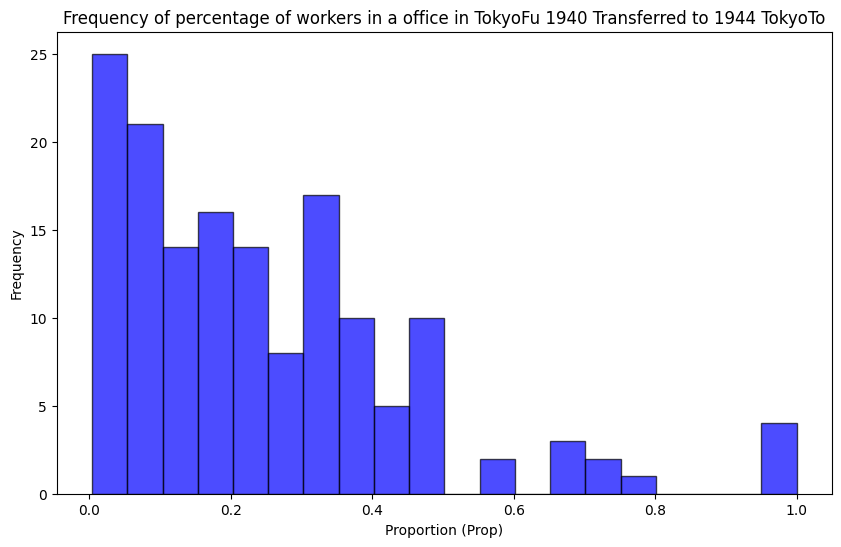
\includegraphics[width = \textwidth]{Background/TokyoFuTransfer.png}
        \label{fig:enter-label}
    \end{figure}
\end{frame}

